\makeatletter
\def\input@path{{../../}}
\makeatother
\documentclass[../../main.tex]{subfiles}

\graphicspath{
  {../../img/}
  {../img/}
  {img/}
}

\begin{document}
	\section{Необходимое условие ЛЭФНП}
	Рассмотрим ФНП $u = f (x)$,
	где $x = (x_1, \ldots, x_n) \in D \subset \R^n$.
	
	Внутрення точка $x_0 = (x_{0 1}, \ldots, x_{0n}) \in D$
	называется \emph{точкой строгого локального минимума (максимума)}
	$f(x)$,
	если
	\[
		\exists V (x_0) \subset D,
		\forall x \in \dot{V} (x_0)
		= V (x_0) \setminus \{x_0\}
		\implies f (x_0) < f (x)
		\Big(f (x) < f (x_0)\Big).
	\]
	Если $\forall x \in V (x_0)$ мы можем гарантировать
	только нестрогие неравенства $f (x_0) \leqslant f (x)
	\\ \displaystyle
	\Big(f (x) \leqslant f (x_0)\Big)$,
	то $x_0$ называется просто \emph{точкой локального минимума (максимума)}.
	
	Общее название таких точек
	--- \emph{точки локального экстремума} для $f (x)$.
	
	Значение $f (x)$ в точке локального экстремума $x_0$
	соответственно будем обозначать
	$f_{min} = f (x_{min})$ и $f_{max} = f (x_{max})$
	и называть \emph{экстремальными значениями} ЛЭФНП.
	
	\begin{exmp}
		Рассмотрим Ф2П
		\[
		\begin{cases}
			u = f (x, y) = x^2 + y^2, \\
			\forall (x, y) \in \R^2. \\
		\end{cases}
		\]
		Для этой функции в пространстве $\R^3$ графиком $\Gamma_f$
		будет являться поверхность $z = x^2 + y^2$,
		соответствующая однополостному параболоиду в ДПСК $Oxyz$.
		\[
			\forall (x, y) \ne (0, 0)
			\implies
			f (x, y) = x^2 + y^2 > 0 = f (0, 0),
		\]
		поэтому точка $M_0 (0, 0) \in \R^2$
		будет являться точкой строгого локального минимума рассматриваемой Ф2П,
		при этом $f_{min} = f (M_0) = 0$.
		
		В данном случае
		этот минимум является не только локальным, но и глобальным.
		
		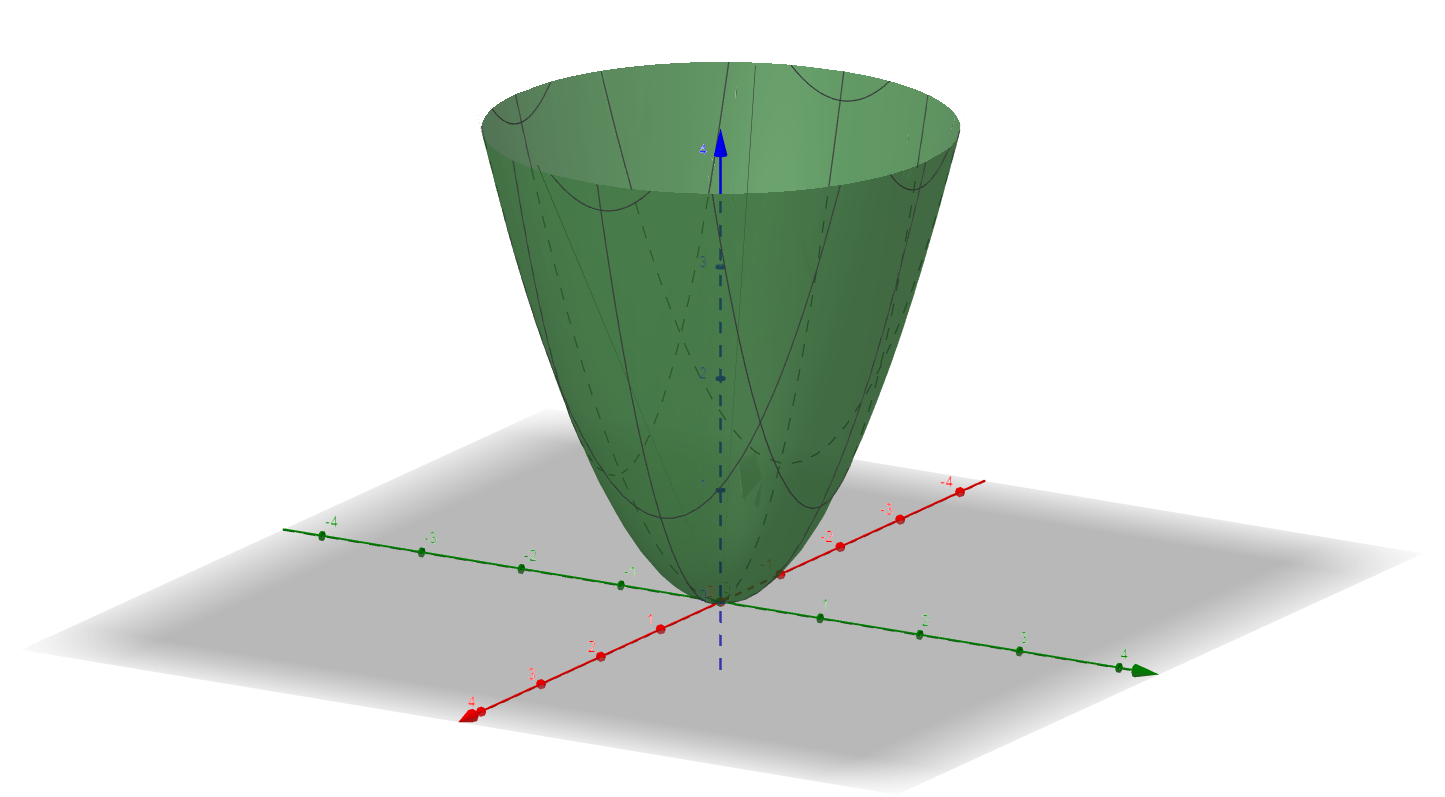
\includegraphics[width=0.9\linewidth]{Ellyptic_paraboloid}
		
	\end{exmp}
	
	Для определения локального экстремума на языке приращений,
	придадим внутренней точке $x_0 \in D$
	произвольные приращения $\D x \in \R^n$ так,
	чтобы $(x_0 + \D x) \in D$.
	Тогда, учитывая, что $\D f (x_0)
	= f (x_0 + \D x) - f (x_0)$,
	в случае, когда $x_0 = x_{min}$, получим
	$f (x_0 + \D x) - f (x_0) \geqslant 0
	\implies
	\D f (f_0) \geqslant 0$.
	Аналогично, если $x_0 = x_{max}$,
	то тогда $\D f (x_0) \leqslant 0$.

	Таким образом, $x_0$ --- точка локального экстремума ФНП
	тогда и только тогда, когда
	приращение функции $\D f (x_0)$ на допустимом
	произвольном $\D x \in \R^n$ сохраняет один и тот же знак.
	
	В случае, когда для допустимых произвольных $\D x \ne 0 \implies
	\D f (x_0) > 0 \displaystyle
	\Big(\D f (x_0) < 0\Big)$
	имеем в $x_0$ строгий локальный минимум (максимум).
	
	\begin{thm}[Необходимое условие ЛЭФНП]
		Пусть ФНП
		\[
		\begin{cases}
			u = f (x), \\
			x = (x_1, \ldots, x_n) \in D \subset \R^n; \\
		\end{cases}
		\]
		дифференцируема в некоторой окрестности $V (x_0) \subset D$
		внутренней точки $x_0 \in D$. Если эта $x_0$ является экстремальной
		для $f (x)$, то $x_0$ --- стационарная точка
		для $f (x)$, т.е. для произвольных допустимых
		\begin{equation}
		\label{nec cond loc extr}
			\forall dx = \D x \in \R^n \implies df (x_0) = 0.
		\end{equation}
	\end{thm}
	\begin{proof}
		Придав точке $x_0 \in V (x_0) \subset D$
		произвольное приращение \\
		$\D x = (\D x_1, \ldots, \D x_n) \in \R$ так,
		чтобы $(x_0 + \D x) \in V (x_0)$,
		наряду с общим приращением функции
		$\D f (x_0) = f (x_0 + \D x) - f (x_0)$,
		рассмотрим для фиксированного $k = \overline{1, n}$
		соответствующее специальное приращение
		$\D_k x = \left(0, \ldots, 0,
		\underbracket{\D x_k}_{k\text{-е место}}, 0, \ldots, 0\right)$,
		для которого
		$(x_0 + \D_k x)
		= \left(x_{0 1}, \ldots, x_{0, k - 1}, x_{0 k} + \D x_k,
		x_{0, k + 1}, \ldots, x_{0 n}\right) \in V (x_0)$.
		
		В результате, получим соответствующие специальные приращения
		рассматриваемой функции по $k$-й координате
		$\D_k f (x_0)
		= f (x_0 + \D x) - f (x_0)$.
		Если $x_0$ --- точка локального минимума (максимума)
		для $f (x)$, то $\D f (x_0) \geqslant 0
		\displaystyle
		\Big(\D f (x_0) \leqslant 0\Big)$,
		откуда следует, что $\D_k f (x_0) \geqslant 0
		\displaystyle
		\Big(\D_k f (x_0) \leqslant 0\Big)$,
		т.е. точка $t_k = x_{0 k}$ будет точкой локального минимума (максимума)
		Ф1П $F_k (t)
		= f (x_{0 1}, \ldots, x_{0, k - 1}, t,
		x_{0, k+1}, \ldots, x_{0 n})$,
		так как здесь 
		\[
			\D F_k (t_k)
			= F_k (x_{0 k} + \D t) - F (x_{0 k})
			= \D_k f (x_0) \geqslant 0.
		\]
		Используя далее необходимое условие локального экстремума Ф1П получим,
		что точка $t_k = x_{0 k}$ является для $F_k (t)$
		стационарной, т.е. 
		\[
			F'_k (t_k) = 0.
		\]
		Отсюда, учитывая, что 
		\[
			F'_k (t_k)
		= \pderiv{f (x_0)}{x_k}, k = \overline{1, n},
		\]
		имеем
		\[
			df (x_0)
			= \sum_{k = 1}^{n}
			\underbracket{\pderiv{f (x_0)}{x_k}}_{= 0} dx_k
			= 0.
		\]
	\end{proof}
	\begin{rem}
		Как и для Ф1П, условие \eqref{nec cond loc extr} в общем случае
		лишь необходимо для экстремальности $x_0$, так как не всякая
		стационарная точка может быть экстремальной. \\
		Например, для Ф2П
		\[
		\begin{cases}
			u = f (x, y) = x^2 - y^2, \\
			(x, y) \in \R^2; \\
		\end{cases}
		\]
		из системы
		\[
		\begin{cases}
			f'_x = 2x = 0, \\
			f'_y = 2y = 0; \\
		\end{cases}
		\]
		получим, что точка $M_0 (0, 0)$ --- стационарная,
		$df (M_0) = 0$,
		но здесь она не будет экстремальной, так как на специальных приращениях
		$(\D x, \D y) \in \R^2$ имеем
		\begin{enumerate}
			\item[а)]
			если
			\[
			\begin{cases}
				\D x = 0, \\
				\D y \ne 0; \\
			\end{cases}
			\]
			то
			\[
				\D f (M_0)
				= f (0, \D y) - f (0, 0)
				= -y^2 < 0;
			\]
			
			\item[б)]
			\[
			\begin{cases}
				\D x \ne 0, \\
				\D y = 0; \\
			\end{cases}
			\implies
			\D f (M_0)
			= x^2 > 0.
			\]
		\end{enumerate}
		Значит, $\forall V (M_0) \subset \R^2$ приращение функции
		не сохраняет один и тот же знак, значит, стационарная точка $M_0$
		не будет экстремальной.
	\end{rem}
\end{document}
